\section{Output}

The output of Complexity Zoology is an HTML file that displays the logical
consequences of the information in the input file. The ouput shows a diagram for
each world $W$ that indicates the distinct classes in $W$ and the relationships
between them.

Each of the six worlds that Complexity Zoology understands can be viewed in the
output file. For each world $W$, there is a diagram for the transitive dual
$W^*$ indicating the inclusions that are true in $W^*$. A black arrow from
$\sC_1$ to $\sC_2$ indicates that $\sC_1\subseteq_{W^*}\sC_2$ and
$\co\cdot\sC_1\subseteq_{W^*}\sC_2$, a blue arrow indicates that
$\sC_1\subseteq_{W^*}\sC_2$, a red arrow indicates that
$\co\cdot\sC_1\subseteq_{W^*}\sC_2$, and a green arrow indicates that
$\cocap\cdot\sC_1\subseteq_{W^*}\sC_2$. Complexity Zoology draws the fewest
arrows necessary to describe the structure of $W^*$. Specifically, the system
describes whether an arrow should be drawn from $\sC_1$ to $\sC_2$ according to
the following rules:
\begin{enumerate}
\item Let $\sC_1\leq_1\sC_2$ denote the relation ``$\sC_1\subseteq_{W^*}\sC_2$
  or $\co\cdot\sC_1\subseteq_{W^*}\sC_2$.'' Let $\sC_1\leq_2\sC_2$ denote the
  relation $\cocap\cdot\sC_1\subseteq_{W^*}\sC_2$. Denote the Hasse relation of
  $\leq_j$ by $\leq_j^\prime$ so that, for example, $\sC_1\leq_1^\prime\sC2$
  indicates that $\sC_1\leq\sC_2$ and there is no $\sC_3$ distinct from $\sC_1$
  and $\sC_2$ such that $\sC_1\leq_1\sC_3\leq\sC_2$.
\item An arrow is drawn from $\sC_1$ to $\sC_2$ if and only if
  $\sC_1\leq_1^\prime\sC_2$ or $\sC_1\leq_2^\prime\sC_2$.
\item Suppose that, by (2), an arrow is to be drawn from $\sC_1$ to $\sC_2$. If
  $\sC_1\subseteq_{W^*}\sC_2$ and $\co\cdot\sC_1\subseteq_{W^*}\sC_2$, color the
  arrow black. If $\sC_1\subseteq_{W^*}\sC_2$ but not
  $\co\cdot\sC_1\subseteq_{W^*}\sC_2$, color the arrow blue. If
  $\co\cdot\sC_1\subseteq_{W^*}\sC_2$ but not $\sC_1\subseteq_{W^*}\sC_2$, color
  the arrow red. If the arrow is not to be colored black, blue, or red, then
  color the arrow green.
\end{enumerate}

So far, the diagrams for $W$ and its transitive dual $W^*$ are identical. They
are distinguished by the fact that they are active diagrams: by clicking on the
node in the diagram corresponding to the class $\sC_1$, all nodes in the diagram
are colored. Assuming the node for a first class $\sC_1$ has been clicked, the
node for a second class is colored in as follows:
\begin{itemize}
\item The color of the left side of the node indicates the status of
  $\sC_1\subseteq_W\sC_2$.
\item The color of the right side of the node indicates the status of
  $\co\cdot\sC_1\subseteq_W\sC_2$.
\item The color of the middle of the node indicates the status of
  $\cocap\cdot\sC_1\subseteq_W\sC_2$. (If the status of $\sC_1\subseteq\sC_2$ or
  $\co\cdot\sC_1\subseteq\sC_2$ implies the status of
  $\cocap\cdot\sC_1\subseteq\sC_2$, then there is no middle color, and only the
  left and right halves of the node are colored.)
\end{itemize}
Green indicates that the inclusion has been proven, red indicates that the
inclusion has been disproven, yellow indicates that the inclusion is open, and
gray indicates that the status of the inclusion is unknown to Complexity
Zoology. Different shades of gray are used to indicate the type of unknown:
green-tinted for provable, red-tinted for disprovable, and untinted for
completely unknown.

\begin{figure}[htb]
  \center{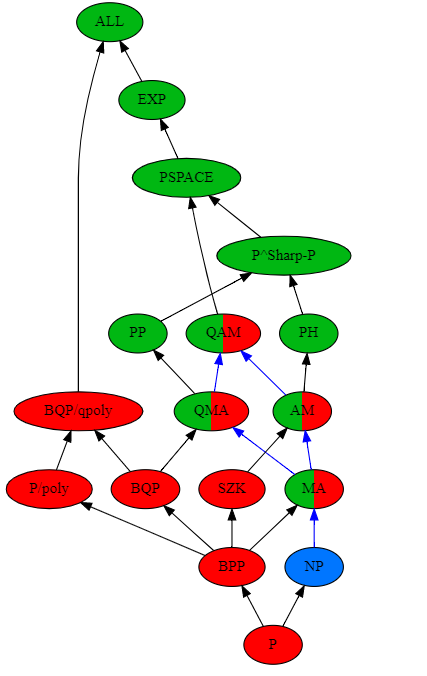
\includegraphics[width=4in]
  {simplified-graph-NP-selected.png}}
  \caption{\label{NP-selected} A sample diagram in the ``all oracles'' world in which 
  $\NP$ is selected. The blue node is selected, a green node indicates that the selected 
  class lies inside the node's class, and a red node indicates that the selected class 
  does not lie inside the node's class. The color on the left side of a node corresponds 
  to the class written in the bubble, while the color on the right corresponds to the 
  complement of the written class. Blue arrows denote containment, while black arrows 
  denote symmetric containment.}
\end{figure}

Finally, a table below the diagram lists alternate names for each complexity
class in $W^*$. In other words, for each class $\sC_1$ that appears in the
diagram, the table lists classes $\sC_1$ for which $\sC_1\subseteq_{W^*}\sC_2$
and $\sC_2\subseteq_{W^*}\sC_1$. Complexity Zoology uses its internal hierarchy
of preferred names to determine which name for a complexity class should appear
in the diagram, choosing arbitrarily between the possibilities having equal
preference.